\begin{center}
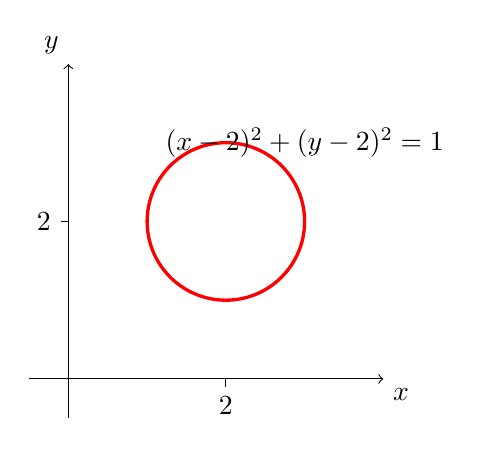
\begin{tikzpicture}
\begin{scope}
    %——————————————————————————————————————————————
    % Ejes de R^2
    %——————————————————————————————————————————————
    % Eje x: desde x=-0.5 hasta x=4
    \draw[->] (-0.5,0) -- (4,0) node[below right] {$x$};
    % Eje y: desde y=-0.5 hasta y=4
    \draw[->] (0,-0.5) -- (0,4) node[above left]  {$y$};
  
    %——————————————————————————————————————————————
    % Circunferencia centrada en (2,2) con radio 1
    %——————————————————————————————————————————————
    % Color rojo, grosor "very thick"
    \draw[red, very thick] (2,2) circle [radius=1];
  
    %——————————————————————————————————————————————
    % Marcas de -delta y +delta (en este caso 2) sobre cada eje
    %——————————————————————————————————————————————
    % Tick en x=2
    \draw (2,0) -- ++(0,-0.1) node[below] {$2$};
    % Tick en y=2
    \draw (0,2) -- ++(-0.1,0) node[left]  {$2$};
  
    %——————————————————————————————————————————————
    % Etiqueta con la ecuación de la circunferencia
    %——————————————————————————————————————————————
    \node at (3,3) {$(x-2)^2 + (y-2)^2 = 1$};
  \end{scope}
\end{tikzpicture}
\end{center}